% Knowledge base and Embedding sections (Hasan Latief). Needs \usepackage{booktabs,graphicx}.
% Every number here comes from experiments/results.md (generated by summarize_runs.py).

\subsection{Knowledge base}

\paragraph{Datasets.}
We use the three BEIR corpora from the PoisonedRAG paper. NQ (2,681,468 passages) and HotpotQA
(5,233,329 passages) are both made of English Wikipedia passages, so together they are the Wikipedia
knowledge base described in our proposal. MS-MARCO (8,841,823 passages) is built from web search results.
We keep it as a non-Wikipedia contrast. We did not use the 21M-passage Wikipedia dump: encoding it on our
GPU (a GTX 1660) would take about 87 hours and 64\,GB of embeddings.
The target questions are the first 30 of the authors' 100 per dataset (10 per iteration, 3 iterations),
with their GPT-4 attack texts. Their ground-truth documents come from the BEIR qrels: the test split for
NQ and HotpotQA, and the train split for MS-MARCO, because that is where its target questions are (as in
the authors' \texttt{main.py}). The BEIR download server was unreachable, so HotpotQA and MS-MARCO were taken from the
\texttt{BeIR/*} mirrors on Hugging Face. Their document counts match the paper's Table~14 exactly.

\paragraph{Attack.}
We use the black-box PoisonedRAG attack: for each target question, $N=5$ attack texts, each made of the
question followed by the authors' GPT-4 text. All $M \times N = 50$ attack texts of an iteration are in the
knowledge base at once, and the retriever returns the top $k=5$. We report poison F1 (precision and recall
are equal because $k=N$), the poison hit rate (at least one attack text in the top-5), and the clean hit rate
(a ground-truth document in the top-5).

\paragraph{Varying the knowledge-base size.}
A subsampled knowledge base of size $S$ holds every ground-truth document of the 30 targets plus a seeded
random sample (seed 12) of other documents, up to $S$ in total. We encode it live and search it exactly
(brute-force dot product on the CPU), so there is no approximate-search error. We use $S \in \{10^4, 10^5,
5\times10^5\}$. For the full corpora, Contriever's clean ranking comes from the authors' cached top-100, merged with
attack-text scores we compute ourselves. Because the subsample always keeps the ground-truth documents, the clean hit
rate at small $S$ is an upper bound and should not be read as a measure of retriever quality. Poison F1 is the
quantity we compare across sizes.

\subsection{Embedding (retrievers)}

\paragraph{Retrievers.}
\begin{itemize}
  \item \textbf{Contriever} (\texttt{facebook/contriever}): BERT-base, mean pooling, 768 dimensions,
        dot product. This is the paper's default retriever.
  \item \textbf{ANCE} (\texttt{msmarco-roberta-base-ance-firstp}): RoBERTa-base, [CLS] pooling, a linear
        layer and LayerNorm, 768 dimensions, dot product. The paper also tests it (Table~5).
  \item \textbf{gte-small} (\texttt{thenlper/gte-small}): a 33M-parameter BERT, mean pooling and L2
        normalisation, 384 dimensions, cosine similarity. This is our addition. It is a smaller, newer
        general-purpose embedder and ranks higher than the other two on public retrieval benchmarks.
\end{itemize}

\paragraph{Sanity checks.}
For each dataset we re-encoded the 30 target questions and their cached top-5 documents and compared our
Contriever scores with the authors' cached scores. The largest difference is $7.2\times10^{-7}$ (NQ),
$6.0\times10^{-7}$ (HotpotQA) and $9.5\times10^{-7}$ (MS-MARCO), so mixing cached and live scores is
sound. For ANCE and gte-small, our batched encoder matches \texttt{SentenceTransformer.encode} to within
$1.4\times10^{-6}$ and $1.1\times10^{-7}$. This check caught a bug: our library version (transformers 5) loads
gte-small in its stored fp16 format, which gave embedding norms of 0.9998. We now cast every model to
fp32. In every run without an attack, the poison F1 is exactly 0, so the metric never counts clean documents as attack texts.

\paragraph{Results.}
Table~\ref{tab:kb-emb} and Figure~\ref{fig:kb-emb} show the results. Our full-corpus Contriever runs replicate
the paper. With the paper's 100 targets we get F1 0.958 on NQ, 0.998 on HotpotQA and 0.894 on MS-MARCO,
against the paper's 0.96, 1.0 and 0.89.

\begin{table}[t]
  \centering\small
  % Generated by summarize_runs.py; needs \usepackage{booktabs}
\begin{tabular}{llrrrr}
\toprule
Dataset & Retriever / KB size & Attack F1 & Poison hit & Clean hit (no attack) & Clean hit (attacked) \\
\midrule
NQ (Wikipedia) & Contriever, 10k & 1.000 & 1.00 & 0.93 & 0.00 \\
 & Contriever, 100k & 1.000 & 1.00 & 0.87 & 0.00 \\
 & Contriever, 500k & 0.987 & 1.00 & 0.57 & 0.00 \\
 & Contriever, full (2.68M) & 0.953 & 1.00 & 0.20 & 0.00 \\
 & ANCE, 10k & 0.993 & 1.00 & 0.97 & 0.03 \\
 & ANCE, 100k & 0.993 & 1.00 & 0.93 & 0.03 \\
 & ANCE, 500k & 0.993 & 1.00 & 0.87 & 0.03 \\
 & gte-small, 10k & 0.987 & 1.00 & 1.00 & 0.07 \\
 & gte-small, 100k & 0.987 & 1.00 & 1.00 & 0.07 \\
 & gte-small, 500k & 0.987 & 1.00 & 0.97 & 0.07 \\
 & gte-small, full (2.68M) & 0.933 & 1.00 & 0.77 & 0.03 \\
\midrule
HotpotQA (Wikipedia) & Contriever, 10k & 0.993 & 1.00 & 1.00 & 0.03 \\
 & Contriever, 100k & 0.993 & 1.00 & 0.93 & 0.03 \\
 & Contriever, 500k & 0.993 & 1.00 & 0.83 & 0.03 \\
 & Contriever, full (5.23M) & 0.993 & 1.00 & 0.77 & 0.03 \\
 & ANCE, 10k & 1.000 & 1.00 & 0.97 & 0.00 \\
 & ANCE, 100k & 1.000 & 1.00 & 0.90 & 0.00 \\
 & ANCE, 500k & 1.000 & 1.00 & 0.83 & 0.00 \\
 & gte-small, 10k & 1.000 & 1.00 & 1.00 & 0.00 \\
 & gte-small, 100k & 1.000 & 1.00 & 1.00 & 0.00 \\
 & gte-small, 500k & 1.000 & 1.00 & 0.93 & 0.00 \\
\midrule
MS-MARCO (web) & Contriever, 10k & 1.000 & 1.00 & 1.00 & 0.00 \\
 & Contriever, 100k & 1.000 & 1.00 & 0.87 & 0.00 \\
 & Contriever, 500k & 0.980 & 1.00 & 0.63 & 0.00 \\
 & Contriever, full (8.84M) & 0.913 & 1.00 & 0.07 & 0.00 \\
 & ANCE, 10k & 0.960 & 1.00 & 0.97 & 0.20 \\
 & ANCE, 100k & 0.960 & 1.00 & 0.97 & 0.20 \\
 & ANCE, 500k & 0.960 & 1.00 & 0.97 & 0.20 \\
 & gte-small, 10k & 0.920 & 1.00 & 1.00 & 0.40 \\
 & gte-small, 100k & 0.920 & 1.00 & 0.90 & 0.40 \\
 & gte-small, 500k & 0.893 & 1.00 & 0.87 & 0.37 \\
\bottomrule
\end{tabular}

  \caption{Poison retrieval with 30 target questions, top-5, $N=5$. Clean hit rate is the fraction of targets with a
    ground-truth document in the top-5, without and with the attack.}
  \label{tab:kb-emb}
\end{table}

\begin{figure}[t]
  \centering
  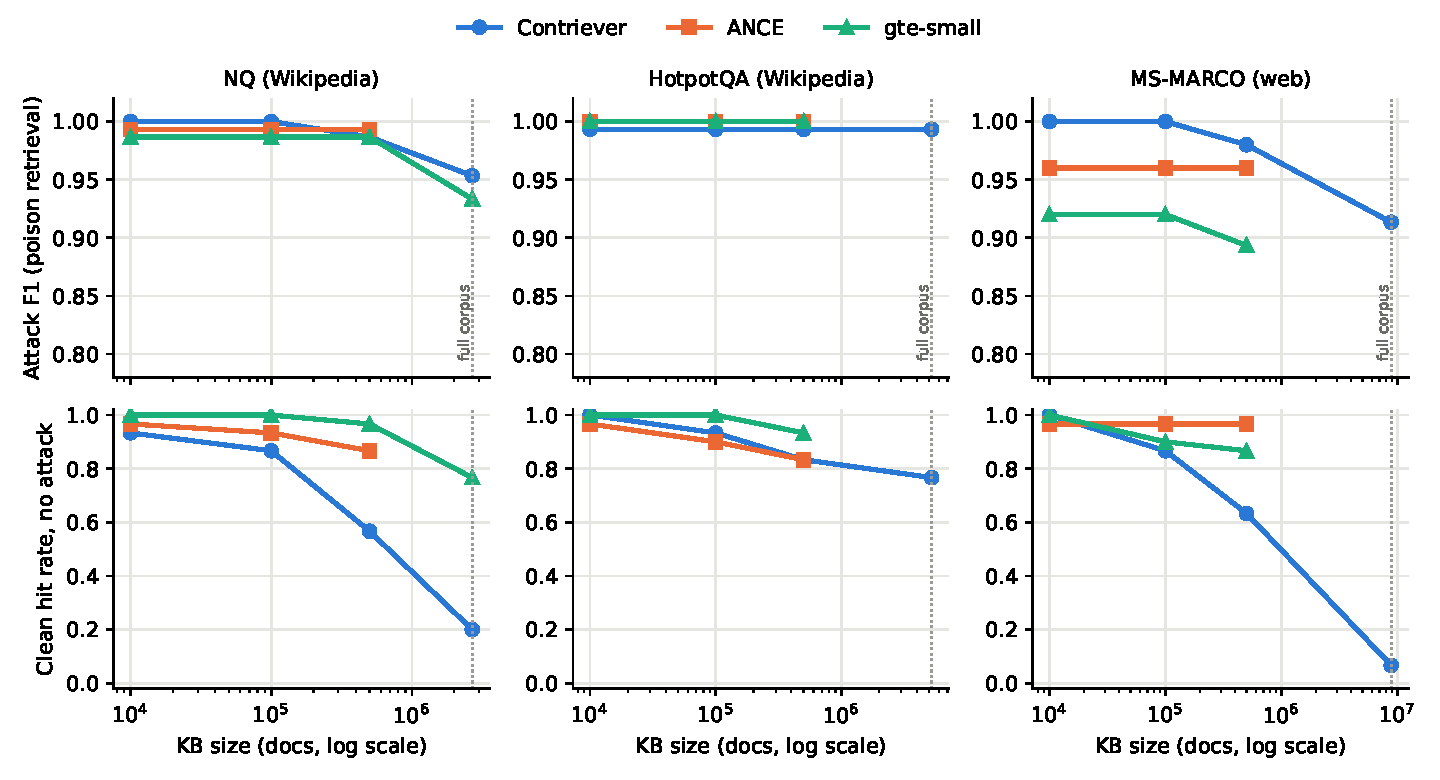
\includegraphics[width=\linewidth]{fig_f1_vs_kb_size.pdf}
  \caption{Attack F1 (top) and clean hit rate without attack (bottom) against knowledge-base size. The dotted line
    marks the full corpus.}
  \label{fig:kb-emb}
\end{figure}

\paragraph{Findings.}
\begin{itemize}
  \item \textbf{All three retrievers are vulnerable.} The poison hit rate is 1.00 in every attack run
        (34 in total). F1 never drops below 0.89 (gte-small on 500k MS-MARCO).
  \item \textbf{A larger knowledge base helps only a little.} From 10k documents to the full corpus,
        Contriever's F1 falls from 1.000 to 0.953 on NQ and from 1.000 to 0.913 on MS-MARCO, and stays at 0.993
        on HotpotQA. Over the same range its clean hit rate falls much faster: from 0.93 to 0.20 on NQ and from 1.00 to 0.07
        on MS-MARCO. More documents make it harder to find the true answer, but barely harder for the attack texts to get in.
        The reason is that each attack text begins with the question itself.
  \item \textbf{A better retriever is not a defence.} gte-small finds the ground-truth document far more often
        than Contriever (0.77 against 0.20 on full NQ), yet its F1 there is 0.933 against 0.953. With the attack,
        its clean hit rate drops to 0.03.
  \item \textbf{Web text is a bit harder to poison than Wikipedia.} On MS-MARCO, gte-small (0.89--0.92) and ANCE
        (0.96) score lower than on the Wikipedia corpora (0.99--1.00). Their clean hit rate under attack stays at
        0.37--0.40 and 0.20, because some short web passages that match the question well still win a top-5 slot.
\end{itemize}

\paragraph{Limitations.}
We use 30 target questions per run, so one missed attack text changes F1 by about 0.007. ANCE and gte-small
run only on subsamples (up to 500k documents), apart from gte-small on full NQ. We test only the black-box
attack and only the retriever; the end-to-end attack success rate with an LLM is covered in another section.
